\section{Velocity Controller}\label{sec:velocityController}
The perpose of the velocity controller is to keep the vehicle at a steady velocity. The PID-controller is the most commonly used - proportional integral differential controller. Often all 3 components are not needed to control the system. Different approaches are explored in the following, starting with the proportional controller.

\subsection{P-Controller}
As seen on \figref{proportionalController} the P-controller is simply a proportional gain which is multiplied in the direct term.
%
\begin{figure}[H]
 	\centering
 	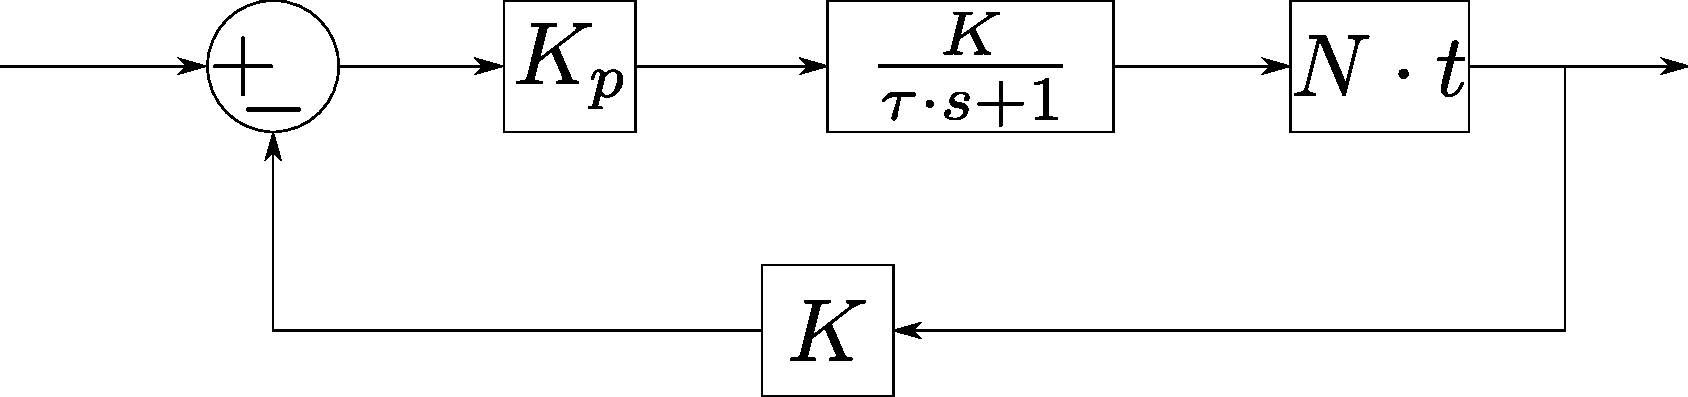
\includegraphics[scale=0.4]{figures/proportionalController.pdf}
 	\caption{Diagram of the proportional controller}
  \label{proportionalController}
\end{figure}
This gives the following closed loop transfer function:
%
\begin{flalign}
  \eq{ \frac{V_{out}}{V_{ref}} }{ \frac{\frac{ K_p \cdot K }{ K_p \cdot K + 1 } }{ \frac{ \tau }{ K_p \cdot K + 1 } \cdot s + 1} }&\nonumber
\end{flalign}
%
From this it is evident that the new system time constant is dependent on the chosen \si{K_p}. The relation is seen directly in the standard form as the coefficient of s:
%
\begin{flalign}
  \eq{ \tau_{closed} }{ \frac{ \tau }{ K_p \cdot K + 1 } }&\nonumber
\end{flalign}
%
So if \si{K_p} is chosen such that it cancels out the gain \si{K} of the plant, allowing for the linear velocity as the input, the time constant will be reduced to half, as will the gain:
\begin{flalign}
  \eq{ \frac{V_{out}}{V_{ref}} }{ \frac{\frac{ \frac{1}{K} \cdot K }{ \frac{1}{K} \cdot K + 1 } }{ \frac{ \tau }{ \frac{1}{K} \cdot K + 1 } \cdot s + 1} }&\nonumber\\
  \eq{ \frac{V_{out}}{V_{ref}} }{\frac{\frac{1}{2}}{\frac{\tau}{2} \cdot s + 1}}&\nonumber
\end{flalign}
%
This means that the P-controller will give an output of half the input, but rise to its set-point twice as fast as the system step without control. This is tested on the vehicle and the response is as expected as seen in \appref{app:proportionalControllerTest}.
%

\subsection{P-Controller with Feed Forward}
Because of its offset the P-controller is not sufficient for reaching and so controlling the decried output velocity. However the P-controller can be improved by manipulating its set-point through use of feed forward, see \figref{proportinalControllerWithFeedforward}.

\begin{figure}[H]
 	\centering
 	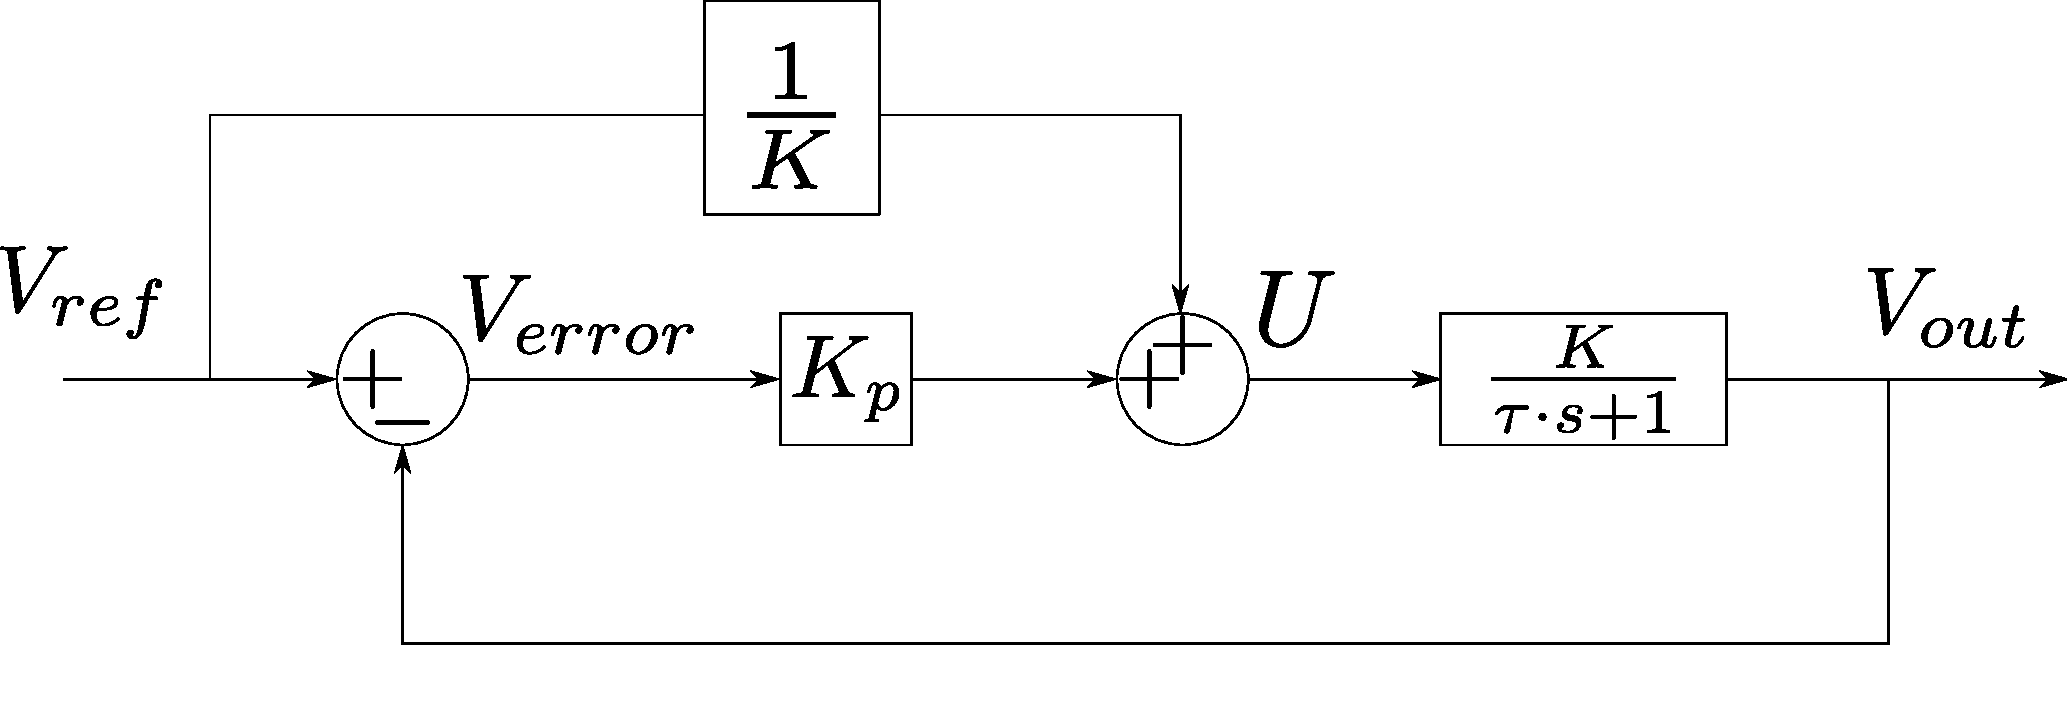
\includegraphics[scale=0.4]{figures/proportionalControllerWithFeedforward.pdf}
 	\caption{Diagram of the proportional controller with feedforward}
 	\label{proportionalControllerWithFeedforward}
\end{figure}

In this design the set-point is changed by forward feeding the desired value of the output \si{V_{ref}} to the input of the plant, summing up with the error fed through the P-controller. The gain on the feed forward makes sure that the value of \si{V_{ref}} is in the same unit as the signal going into the plant, here in volts, \si{U}. Since the system gain \si{K} converts volts into linear velocity, the gain in the forward feed is set to \si{\frac{1}{K}}, which yields the following closed transfer function:

\begin{flalign}
  \eq{ \frac{V_{out} }{V_{ref}} }{ \frac{\frac{K\cdot \frac{1}{K}+K\cdot K_p}{1+K \cdot K_p}}{\frac{\tau}{1+K\cdot K_p}\cdot s + 1 } }&\nonumber\\
  \eq{ \frac{V_{out} }{V_{ref}} }{ \frac{\frac{K\cdot \frac{1}{K}+K\cdot \frac{1}{K}}{1+K \cdot \frac{1}{K}}}{\frac{\tau}{1+K\cdot \frac{1}{K}}\cdot s + 1 } }&\nonumber\\
  \eq{ \frac{V_{out} }{V_{ref}} }{ \frac{1}{\frac{\tau}{2} \cdot s + 1} }&\nonumber
\end{flalign}

From this it is evident

\begin{figure}[H]
 	\centering
 	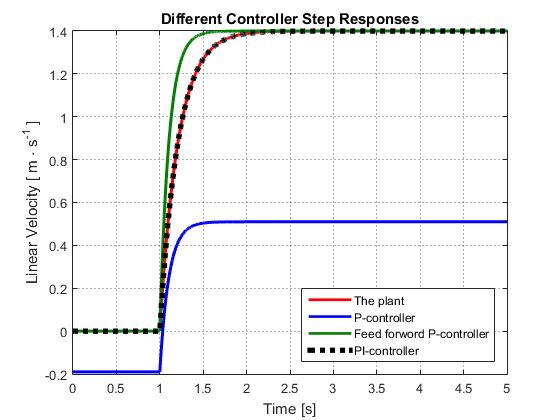
\includegraphics[scale=0.4]{figures/ControllerSteps}
 	\caption{Diagram of the proportional controller}
 	\label{fig:ControllerSteps}
 \end{figure}

\begin{figure}[H]
 	\centering
 	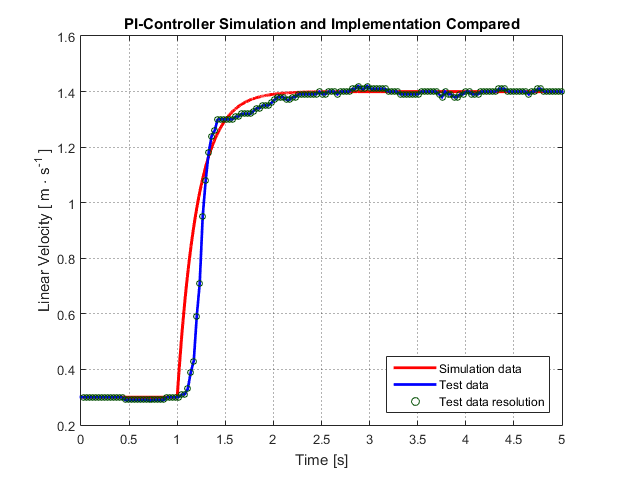
\includegraphics[scale=0.4]{figures/PIcontrollerStepRealVsSim}
 	\caption{Diagram of the proportional controller}
 	\label{fig:PIcontrollerStepRealVsSim}
 \end{figure}




% Comparing step-response, P-controller and P-controller with feed-forward.

 
  
 
% Results:
% Overshoot

% Conclusion: 
% That we need more than a P-controller, because of the overshoot. 




\subsection{PI-Controller}

  \begin{figure}[H]
  	\centering
  	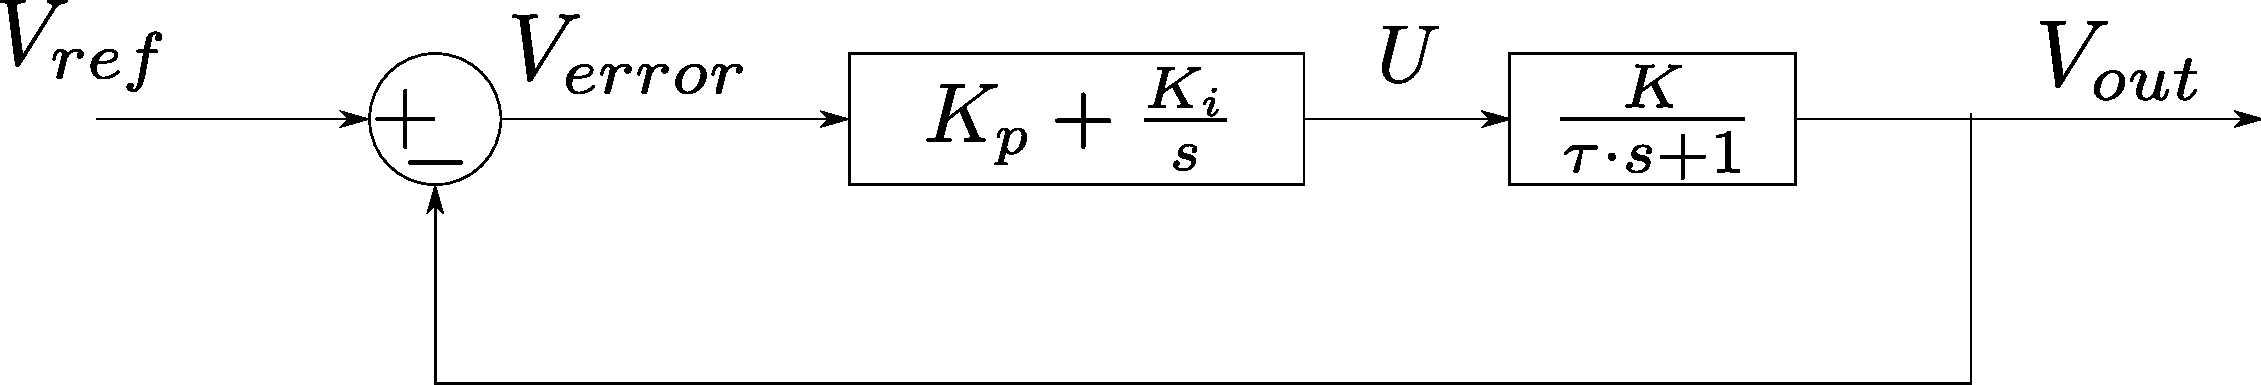
\includegraphics[scale=0.4]{figures/proportionalIntegratorController.pdf}
  	\caption{Diagram of the proportional and Integrator controller without feedforward}
  	\label{proportionalIntegratorController}
  \end{figure}